\section{Modeling \podtm} \label{sec:pod-model}
In this section, we introduce the notion of a \podtm, a distributed protocol where clients can \emph{read} and \emph{write} transactions.
We first define basic data structures and the interface of a \podtm.
We then introduce the basic definition of a \emph{secure \podtm} and its security properties, as well as some additional properties (\emph{timeliness} and \emph{monotonicity}) that it may satisfy, which we later use for some applications.

\begin{definition}[Transaction trace]
    The \emph{transaction trace} of a transaction $\tx \in \zo^*$ is a tuple containing the values $(\tx, \rmin, \rmax, \rconf$, $\txcert)$, which change during the execution of a \podtm protocol.
    We call $\rmin \in \BN$ the \emph{minimum round}, $\rmax \in \BN \cup \{\infty\}$ the \emph{maximum round},
    $\rconf \in \BN \cup \{\bot\}$ the \emph{\confirmed round}, and $\txcert \in \zo^*$ contains some auxiliary data.
    We denote by $\rmax=\infty$ an unbounded maximum round and by $\rconf=\bot$ an undefined \confirmed round.
    We also denote the values in the trace of $\tx$ by $\tx.\rmin, \tx.\rmax, \tx.\rconf$, and $\tx.\txcert$.
\end{definition}

In \podtm-core, \txcert will contain digital signatures used to achieve accountability.

\begin{definition}[Confirmed transaction]
    A transaction with confirmed round \rconf is called \emph{\confirmed} if $\rconf \neq \bot$, and \emph{unconfirmed} otherwise.
\end{definition}

\begin{definition}[Trace set]
A \emph{trace set} $\txSet$ is a set of traces $(\tx, \rmin, \rmax, \rconf, \txcert)$. We say that a transaction $\tx$ \emph{appears} in $\txSet$ when $\exists (\tx, \rmin, \rmax, \rconf, \txcert) \in \txSet$, otherwise we say that a transaction $\tx$ \emph{does not appear} in $\txSet$.
\end{definition}


\begin{definition}[Pod data structure]
    A pod data structure $\Pod$ is a triple $(\txSet, \rperf, \ppcert)$, where \txSet is a trace set, \rperf is a round number, called the \emph{past-perfect round},
    and $\ppcert \in \zo^*$ contains auxiliary data.
\end{definition}

In \podtm-core, \ppcert will also contain signatures used to achieve accountability.
Our construction will allow for deriving $\ppcert$ from all certificates $\txcert$ in $\txSet$, but we define $\ppcert$ explicitly for clarity and generality.
Moreover, \rperf will imply a completeness property on \txSet, defined by the past-perfection safety property of \podtm.
We remark that transactions in \txSet may be \confirmed on unconfirmed.

%We now define the \podtm protocol interface and associated concepts.
\begin{definition}[Interface of a \podtm]\label{def:podinterface}
A \podtm protocol has the following interface.
\begin{itemize}
    \item $\opwrite{\tx}$:
    % \item $\opwrite{\tx} \returns (\rmin, \rmax, \rconf, \txcert)$:
    It writes a transaction \tx to the \podtm.

    \item $\opreadall{} \returns \Pod$:
    It outputs a pod data structure $\Pod = (\txSet, \rperf, \ppcert)$.
    % The second output is called an \emph{equivocation-evidence pod} and can be either $\bot$ or $\tilde{\Pod} = (\tilde{\txSet}, \tilde{\rperf}, \tilde{\ppcert})$.
\end{itemize}
    We say that a client \emph{reads the} \podtm when it calls \opread{}.
    If $\tx$ appears in $\txSet$,
    %$(\tx, \rmin, \rmax, \rconf, \txcert) \in \txSet$
     we say that the client \emph{observes} \tx and, if $\tx.\rconf \neq \bot$, we say that the client \emph{observes \tx as \confirmed}.
\end{definition}

\begin{definition}[Validity of a pod data structure]
    A pod protocol specifies a computable, deterministic, and non-interactive function \opValid{\Pod} that takes as input a pod data structure $\Pod$ and outputs a boolean value.
\end{definition}

% \begin{definition}[Past-perfect round]
% 	Given a set \txSet obtained by an honest client who reads the pod, a round \rperf is \emph{past-perfect} if,
% 	for any transaction $\tx$ that does not appear in $ \txSet$, no honest client will ever observe \tx as confirmed with $\tx.\rconf < \rperf$.
% \end{definition}

\begin{definition}[View of the \podtm]
    We call \emph{view of the} \podtm the output of \opreadall{}, where \opreadall{} is invoked by client \client and the output is produced at round \round,
    and denote it as \podView{\client}{\round}.
    We remark that \round denotes the round when \opread{} outputs, as the client may have invoked it at an earlier round.
    We denote the components of a view as $\podView{\client}{\round}=(\podView{\client}{\round}.\txSet,
    \podView{\client}{\round}.\rperf, \podView{\client}{\round}.\ppcert)$.
    We write $\tx \in \podView{\client}{\round}$ if $\tx$ appears in $\podView{\client}{\round}.\txSet$.
\end{definition}


\begin{definition}[Secure \podtm]\label{def:podsec}
A protocol is a \emph{secure} \podtm if it implements the \podtm interface of Definition~\ref{def:podinterface} and specifies a valid function \opValid{}, such that the following properties hold.

\begin{description}[leftmargin=1mm]
    \item[(Liveness) Validity completeness:]
    If $\podView{\client}{\round}$ is the view of an honest client $\client$ at round $\round$, then $\opValid{\podView{\client}{\round}} = \true$.

    \item[(Liveness) Confirmation within \parConf:]
	Transactions become \confirmed after at most \parConf rounds.
	Formally, if an honest client $\client$ writes a transaction \tx at round \round, then for any honest client $\client'$ (including $\client=\client'$) it holds that $\tx \in \podView{\client'}{\round + \parConf}$ and $\tx.\rconf \neq \bot$.
	% \item[Confirmation within \parConf:]
	% If an honest client writes a transaction \tx at round \round, then it will obtain output $(\tx, \rmin, \rmax, \rconf, \txcert)$, such that $\rconf \neq \bot$, by round $\round + \parConf$.
	% \item[Availability after \parLive:]
	% If an honest client writes a transaction \tx at round \round, then for any honest client $\client$, it holds that $\tx \in \podView{c}{\round + \parLive}$ and $\tx.\rconf \neq \bot$.

	\item[(Liveness) Past-perfection within \parPerf:]
	Rounds become past-perfect after at most $\parPerf$ rounds.
	Formally, for any honest client \client and round $\round \geq \parPerf$,
	it holds that $\podView{c}{\round}.\rperf \geq \round - \parPerf$.

	\item[(Safety) Past-perfection:]
    A valid pod \Pod contains all transactions that may ever obtain a \confirmed round smaller than $\Pod.\rperf$. Formally,
	the adversary cannot output $\Pod_1$ and $\Pod_2$ to the network, such that $valid(\Pod_1) \land valid(\Pod_2)$ and there exists a transaction $\tx$ such that $(\tx, \rmin^1, \rmax^1, \rconf^1, \txcert^1) \in \Pod_1.\txSet$ and $(\tx, \rmin^2, \rmax^2, \rconf^2, \txcert^2) \not\in \Pod_2.\txSet$ and $\rconf^1 < \Pod_2.\rperf$.

	\item[(Safety) Confirmation bounds:] The values $\rmin$ and $\rmax$ bound the \confirmed round that a transaction may ever obtain. Formally,
    the adversary cannot output $\Pod_1$ and $\Pod_2$ to the network, such that $valid(\Pod_1) \land valid(\Pod_2)$ and there exists a transaction $\tx$ such that $(\tx, \rmin^1, \rmax^1, \rconf^1, \txcert^1) \in \Pod_1.\txSet$ and $(\tx, \rmin^2, \rmax^2, \rconf^2, \txcert^2) \in \Pod_2.\txSet$ and $\rmin^1 > \rconf^2$ or $\rmax^1 < \rconf^2$.

\end{description}
\end{definition}


%The \emph{confirmation within \parConf} property gives us that, if an honest client writes a transaction \tx, then \tx will obtain $\rconf \neq \bot$ within \parConf rounds, but it does not tell us \emph{what} that \rconf will be.
%Similarly,
The \emph{confirmation bounds} property gives $\rmin^1 \leq \rconf^2 \leq \rmax^1$, for $\rmin^1, \rmax^1, \rconf^2$ computed by honest clients, but it does not guarantee anything about the values of $\rmin^1$ and $\rmax^1$ (for example, it could trivially be $\rmin^1=0$ and $\rmax^1=\infty$).
To this purpose we define an additional property of \podtm, called \emph{timeliness}.
% , which can be satisfied along with the standard safety and liveness properties of \podtm.
Previous work has observed a similar property as orthogonal to safety and liveness~\cite{EPRINT:TziSriZin23}.

\begin{definition}[\podtm \parTemp-timeliness for honest transactions]\label{def:pod-timely}
    A \podtm protocol is \emph{\parTemp-timely} if it is a secure \podtm, as per Definition~\ref{def:podsec}, and for any honest clients $\client_1,\client_2$, if $\client_1$ writes transaction \tx in round $\round$, then $\client_2$ computes \rmin, \rmax, \rconf for \tx such that:
    % (observe that, from the \emph{confirmation within \parConf} property, \tx will become confirmed):
    \begin{enumerate}
        %\item $\rconf \in (\round, \round + \parTemp]$
        \item $\rmax \in (\round, \round + \parTemp]$
        \item $\rmax - \rmin < \parTemp$, implying that $\rmin \neq 0$ and $\rmax \neq \infty$.
    \end{enumerate}
\end{definition}


Moreover, a \podtm protocol allows the values \rmin, \rmax, \rconf to change during an execution -- for example, clients in construction \podtm-core will update them when they receive votes from replicas.ß
The properties we have defined so far do not impose any restriction on how they evolve.
For this reason, in Appendix~\ref{app:monotonicity} we define the additional property of \podtm \emph{Monotonicity}.

We conclude this section with some visual examples in Figures \ref{fig:temperature} and \ref{fig:example-output}.
% \begin{figure}[h]
%     \centering
%     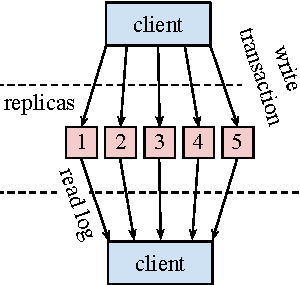
\includegraphics[width=0.35\textwidth]{figures/pod-architecture.pdf}
%     \caption{\todo{Add figure} }
%     \label{fig:example-output}
% \end{figure}


\begin{figure}[ht]
    \begin{minipage}[b]{.48\textwidth}
    \centering
    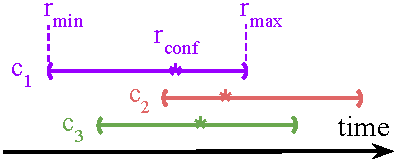
\includegraphics[width=1\textwidth]{figures/pod-temperature.pdf}
    \caption{The same transaction in the view of three different pod clients. Each client assigns it a minimum round \rmin and a maximum round \rmax. If it gets confirmed, the confirmation round \rconf will be
     between these two values. The \rconf that each client locally computes respects the bounds of each other client.}
     \label{fig:temperature}
    \end{minipage}
    \hfill
    \begin{minipage}[b]{.49\textwidth}
    \centering
    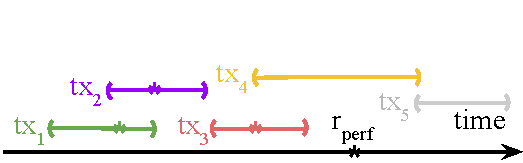
\includegraphics[width=1\textwidth]{figures/pod-example.pdf}
    \caption{A possible view of a single pod client.
    Transactions $\tx_1, \tx_2, \tx_3$ are confirmed, $\tx_4$ is not yet confirmed.
    A client also derives a past-perfect round $\rperf$. No transaction other than $\tx_1, \tx_2, \tx_3, \tx_4$ may  obtain $\rconf \leq \rperf$. There may exist $\tx_5$ for which the client has not received votes, but $\tx_5$ cannot obtain $\rconf \leq \rperf$.
    % Transactions written concurrently, or close to each other, such as $\tx_3$ and $\tx_4$, may not be totally ordered. Transactions written by malicious clients, such as $\tx_5$ may not become confirmed.
    }
    \label{fig:example-output}
    \end{minipage}
\end{figure}



% \subsection {Properties recap}
% This is for us. It summarizes the aforementioned properties and shows which algorithms satisfy them.
% \begin{center}
%     \begin{tabular}{ |l|c|c||c|c|c| }
%         \hline
%                                                                & \multicolumn{2}{c||}{streaming} & \multicolumn{2}{c|}{streaming+gossip}\\
%         \hline
%                                                                & sync  & async  &sync & async \\
%         Confirmation                                           & O& O& O& O\\
%         Pp liveness                                            & O& O& O& O\\
%         Common subset                                          & X& X& O& O\\
%         Common subset for honest tx                            & O& O& O& O\\
%         Conf. stickiness                                       & O& O& O& O\\
%         Correctness of assoc. values                           & O& O& O& O\\
%         Pp correctness                                         & O& O& O& O\\
%         Pp stickiness                                          & O& O& O& O\\
%         \hline
%     \end{tabular}
%     \end{center}
